\documentclass[10pt]{article}
\usepackage[margin=1in]{geometry}
 \usepackage{auto-pst-pdf}
\usepackage{graphicx}
\usepackage{footnote}
%\usepackage{arydshln}
\usepackage{ifpdf}
\ifpdf
  \usepackage{epstopdf}
\fi
\usepackage{multirow}
\usepackage{epsfig}
\usepackage{float}
\usepackage{url}
\usepackage{color}
\usepackage{subfigure}

%\newcommand\solidrule[1][1cm]{\rule[0.5ex]{#1}{.4pt}}
%\newcommand\dashedrule{\mbox{%
%  \solidrule[2mm]\hspace{2mm}\solidrule[2mm]\hspace{2mm}\solidrule[2mm]}}
  
%\usepackage{hyperref}

\begin{document}
\title{Characterizing Execution Times on Realistic Programs}

\author{
Database \& Big Data Systems Laboratory,\\
School of Computer Science and Engineering, \\
Kyungpook National University,\\
Young-Kyoon Suh\\
}
\maketitle

\section{Description}
This document characterizes execution times 
measured on several real-world programs with different input sizes. 
To achieve this characterization, we discuss 
various histograms of execution times, measured in program time (PT), of the programs throughout this document. 
In this work we wish to achieve several goals as follows. 
The first goal is to unravel any structure behind the histograms and present insights into how such structure is formed. 
Another goal is to build a statistical distribution (or model) fitting in the histograms. 
From that distribution, we may reach predicting a concrete execution time considering system noise via 
the model on an arbitrary algorithm with a given input on a real execution environment. 
As a note, the execution times were measured along with the EMPv5~\cite{EMP} protocol. 
%In the protocol, we use taskstats C struct to get measures of a captured process. 
%The taskstat's data is delivered via a netlink socket from the kernel space. 
%The receive buffer for the socket is not robust for many observed processes~\cite{Metrology}. 
%Fortunately, there is an average of 95 processes per iteration of a run, 
%which turns out to be fine with the struct. 
%For a much more number of processes, 
%the use of  {\tt /proc/}[pid]{\tt{/stat}} is preferred, 
%as (i) there are equivalent measures available in the {\tt /proc} filesystem, 
%and (ii) there's little constraint on the use as opposed to taskstats. 

The following section shows histograms for runs on 
different real-world programs with varying input sizes.

\section{Histograms of the Execution Times on Real-World Programs~\label{sec:real-world}} 

In this section we present histogram data 
for two main programs: {\it insertion sort} and {\it matrix multiplication}. 
For the runs of these programs, we varied their input sizes by 2{\small $\times$} 
and measured execution times of the programs over each input size. 

\subsection{Insertion sort~\label{sec:sort}} 
This section shows a series of histograms of an insertion sort program. 
The program repeatedly runs 40 times for a given input size. 
The input size for the program 
varies from 100,000 to 3,200,000 integer elements, which are randomly generated. 
Note that each sort program over a specific input size is termed SORT{\it x}: 
for instance, SORT100 indicates the insertion sort program over 100K elements. 

Figures~\ref{fig:sort1} and ~\ref{fig:sort2} exhibit 
histograms of the execution times measured on the same insertion sort program as 
the input size grows from 100K to 800K elements by the steps of 2x. 
Note that we used one standard deviation in Figure~\ref{fig:sort400_dist} as
a couple of outliers, which were not eliminated by the original protocol, 
resulted in disturbing the rendering of a clean distribution. 

\pagebreak

\begin{figure}[h]
	\centering
	\subfigure[PT frequency on SORT100]{
		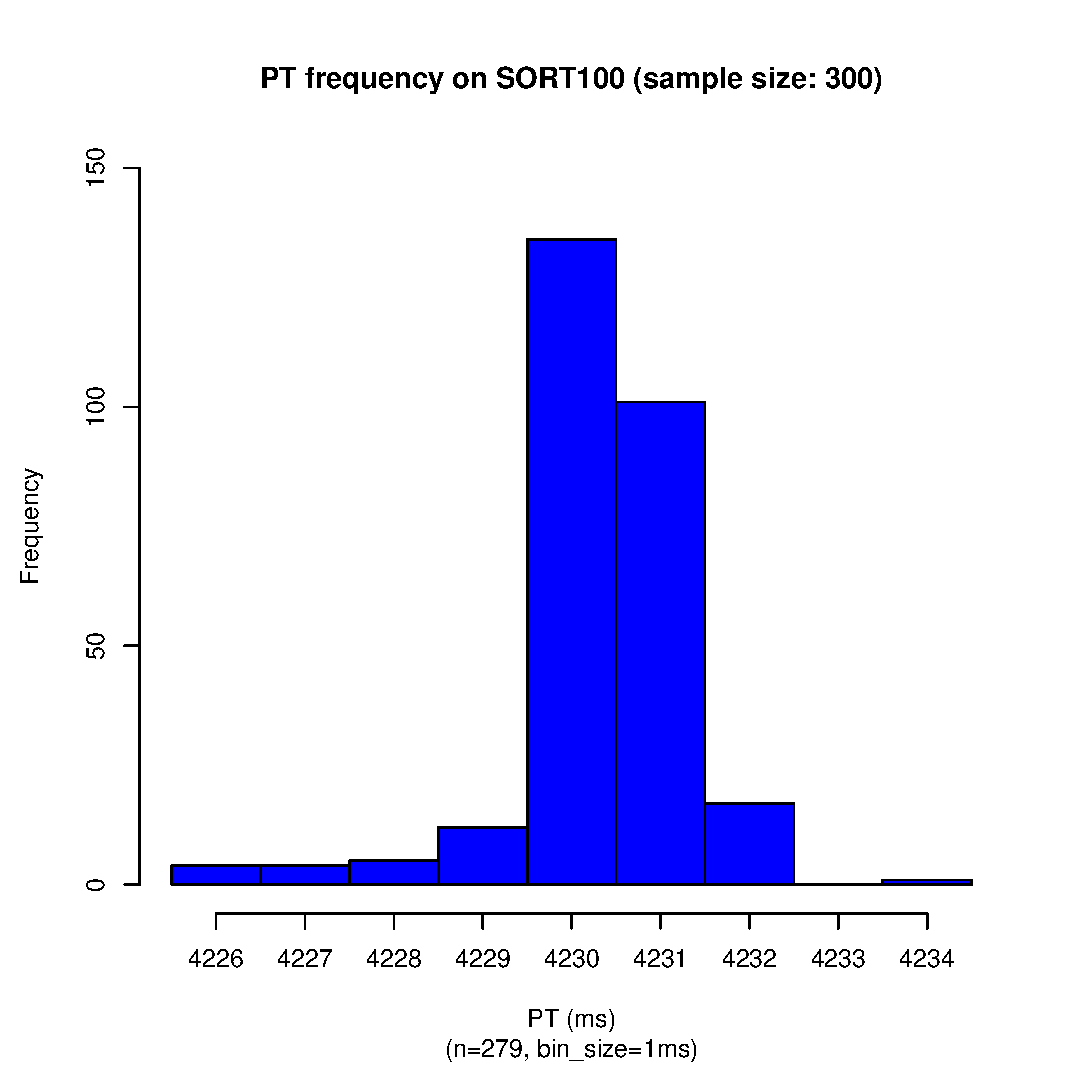
\includegraphics[scale=0.43]{sort100_dist.eps}
		\label{fig:sort100_dist}
	}
	\subfigure[PT frequency on SORT200]{
		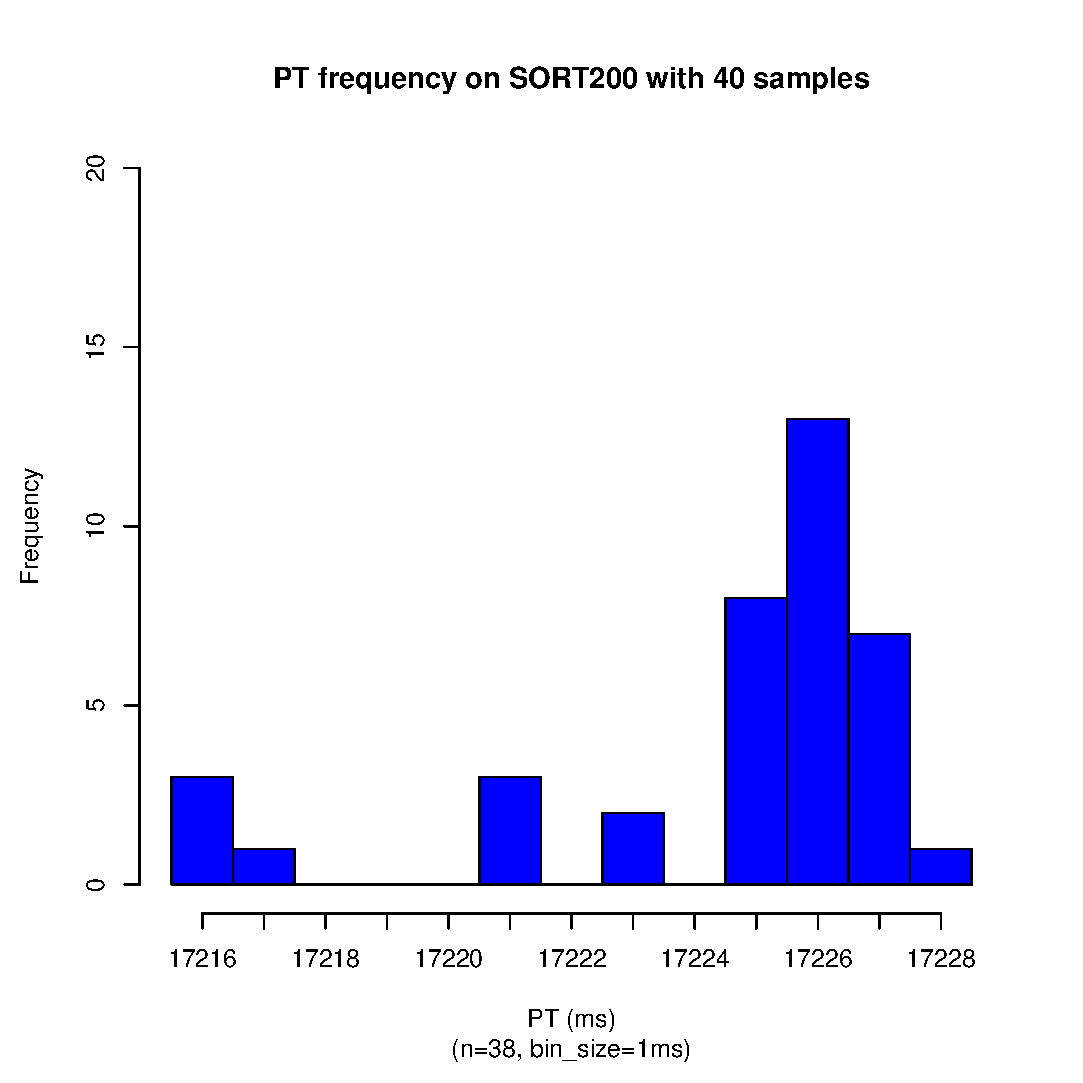
\includegraphics[scale=0.43]{sort200_dist.eps}
		\label{fig:sort200_dist}
	}
	\subfigure[PT frequency on SORT400]{
		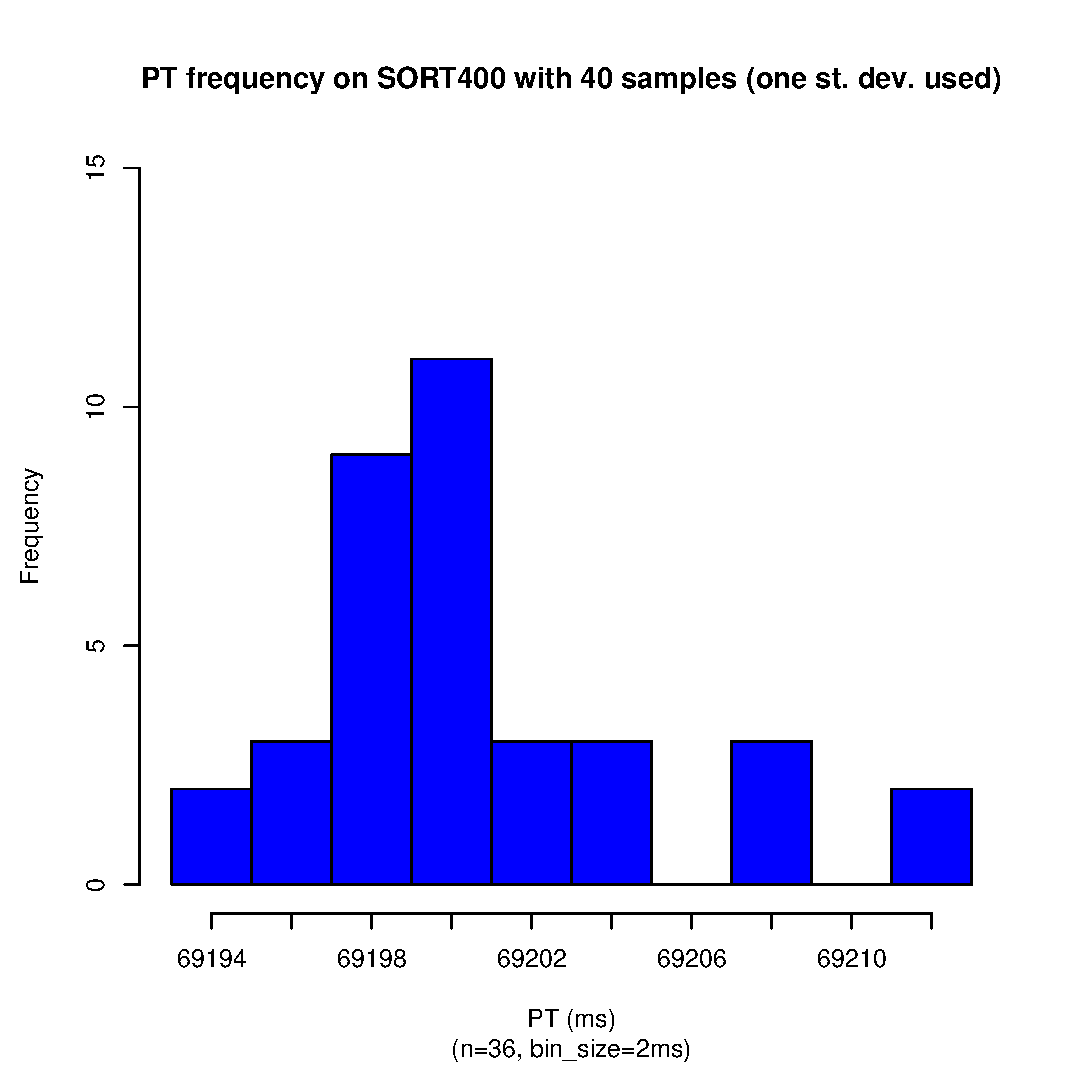
\includegraphics[scale=0.43]{sort400_dist.eps}
		\label{fig:sort400_dist}
	}
	\subfigure[PT frequency on SORT800]{
		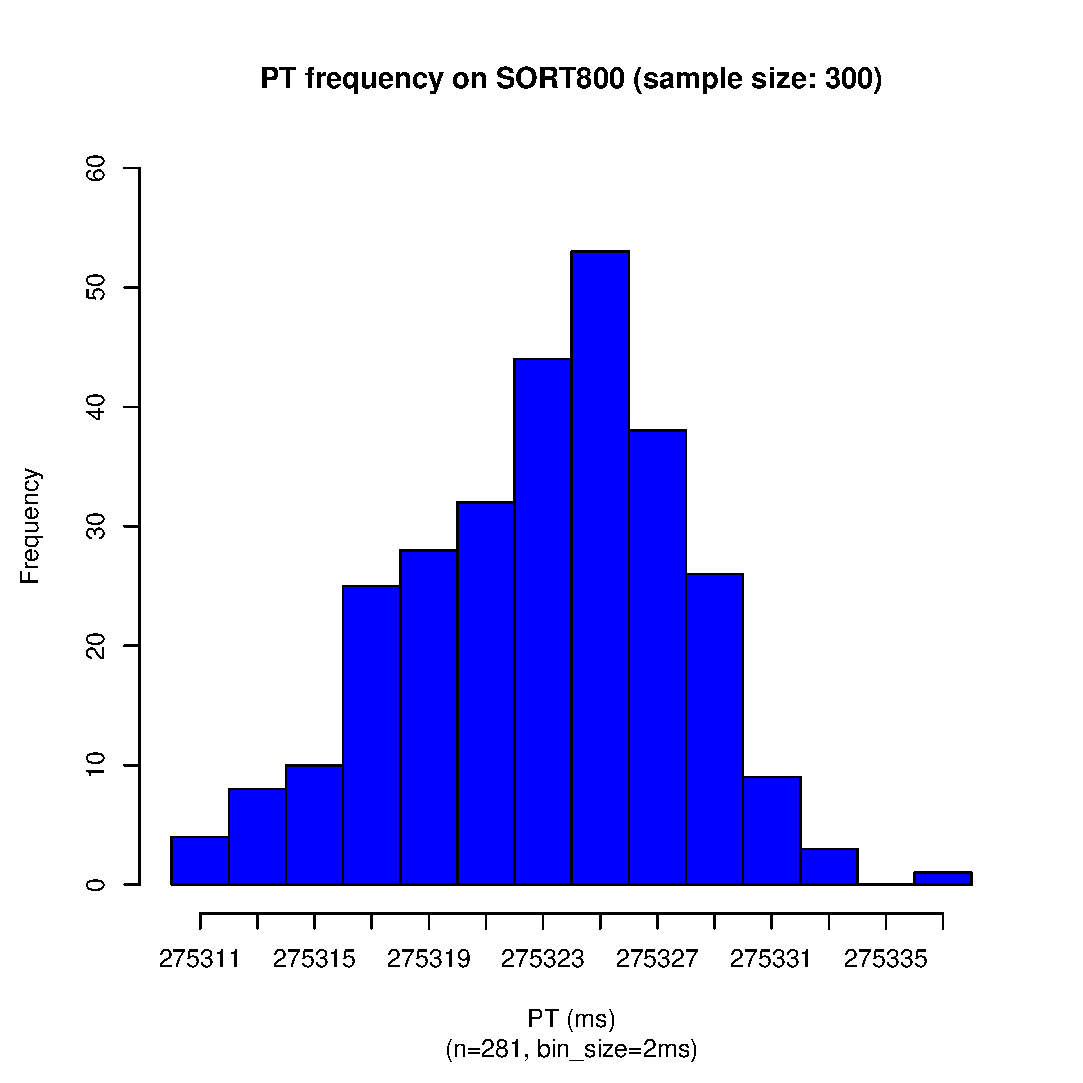
\includegraphics[scale=0.43]{sort800_dist.eps}
		\label{fig:sort800_dist}
	}
	\caption{PT Histograms of SORT100 ... SORT800~\label{fig:sort1}}
\end{figure}

\pagebreak

\begin{figure}[h]
	\centering
	\subfigure[PT frequency on SORT1600]{
		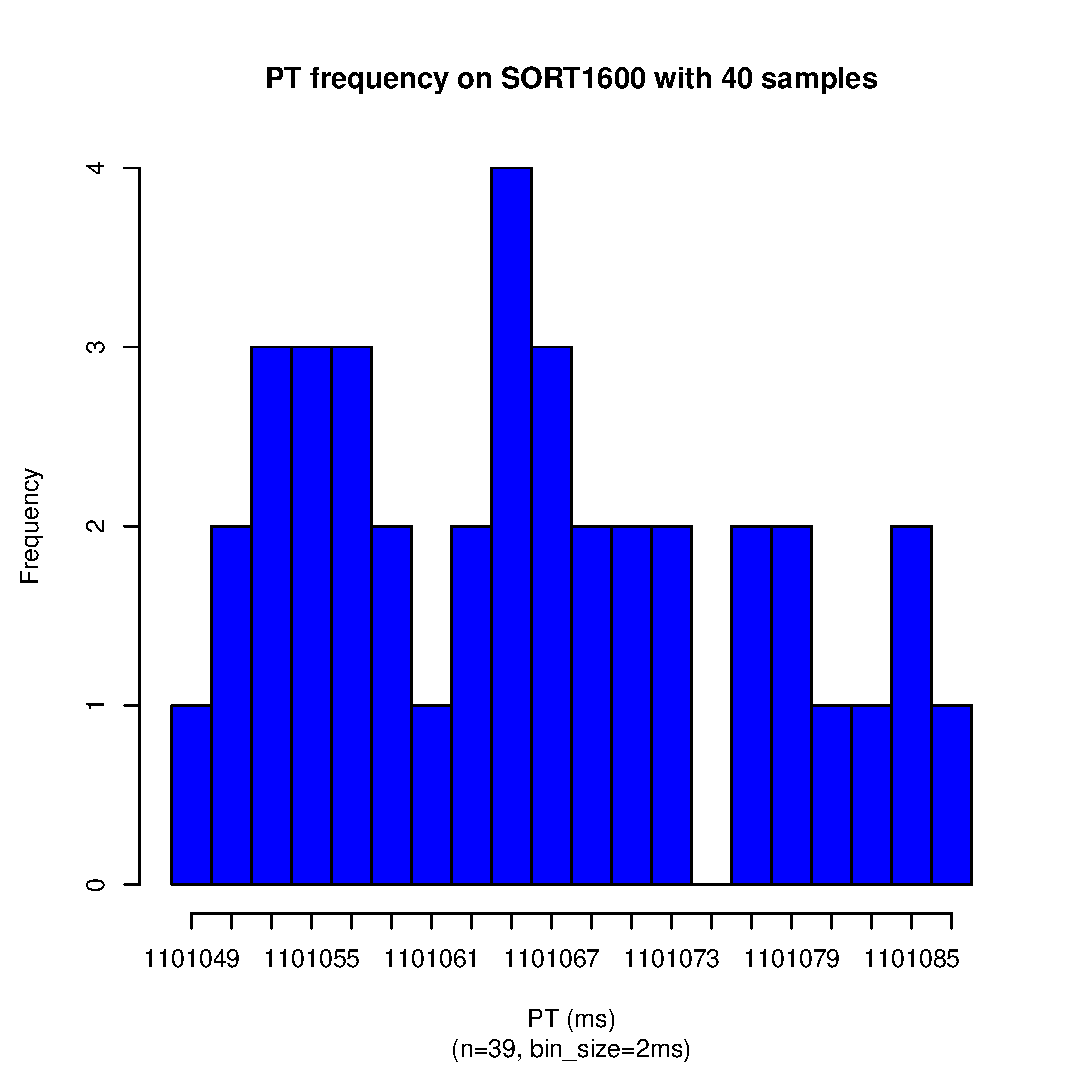
\includegraphics[scale=0.43]{sort1600_dist.eps}
		\label{fig:sort1600_dist}
	}
	\subfigure[PT frequency on SORT3200]{
		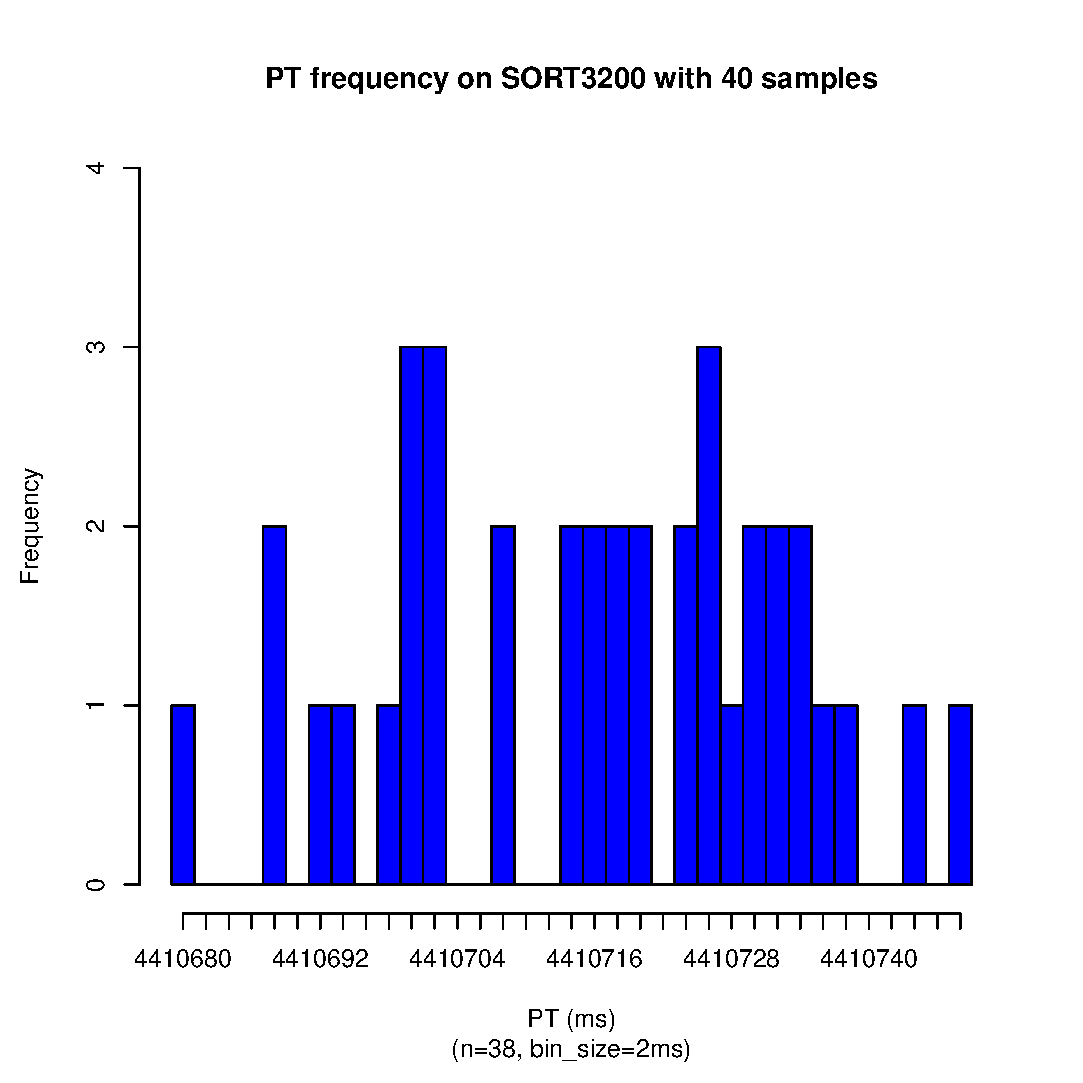
\includegraphics[scale=0.43]{sort3200_dist.eps}
		\label{fig:sort3200_dist}
	}
	\caption{PT Histograms of SORT1600 and SORT3200~\label{fig:sort2}}
\end{figure}

\subsection{Matrix Multiplication~\label{sec:mm}} 

This section shows a series of histograms of 
the execution times of an matrix multiplication program. 
We used the same sample size for each input size of this program: i.e., 40 iterations. 
For simplicity, we used two square matrices for performing their multiplication in the program.  
We also varied the input sizes of each of the two matrices: 
from 1K$\times$1K to 8K$\times$8K integer elements that are also randomly generated. 
Note that each matrix multiplication program for a specific size is called MAT{\it xyyyy}, 
where {\it x} indicates which major, specifically {\em column} vs. {\em row}, is used, and {\it yyyy}, how large a given matrix is. 
For instance, MATC1000 represents a matrix multiplication program 
in column major over two square matrices having 1,000 integer (random) 
elements in a row (and a column). 

\subsubsection{Column Major}

Figure~\ref{fig:matc} shows a series of 
histograms of the execution times measured on 
the same matrix multiplication program in column major 
as the input sizes grows from 1000x1000 to 8000x8000 by the steps of 2{\small $\times$}.. 

\pagebreak

\begin{figure}[h]
	\centering
	\subfigure[PT frequency on MATC1000]{
		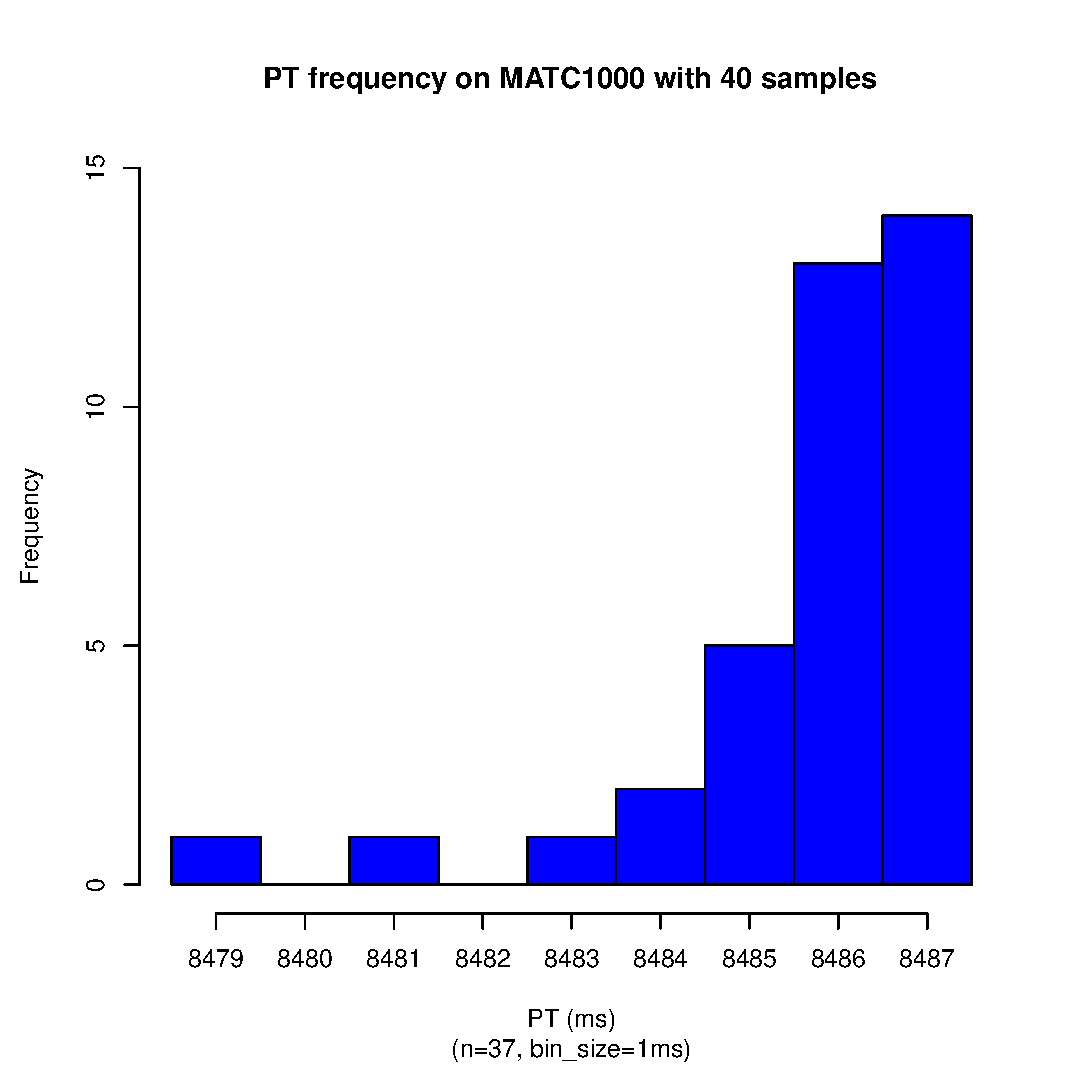
\includegraphics[scale=0.43]{matc1000_dist.eps}
		\label{fig:matc100_dist}
	}
	\subfigure[PT frequency on MATC2000]{
		\includegraphics[scale=0.43]{matc2000_dist.eps}
		\label{fig:matc200_dist}
	}
	\subfigure[PT frequency on MATC4000]{
		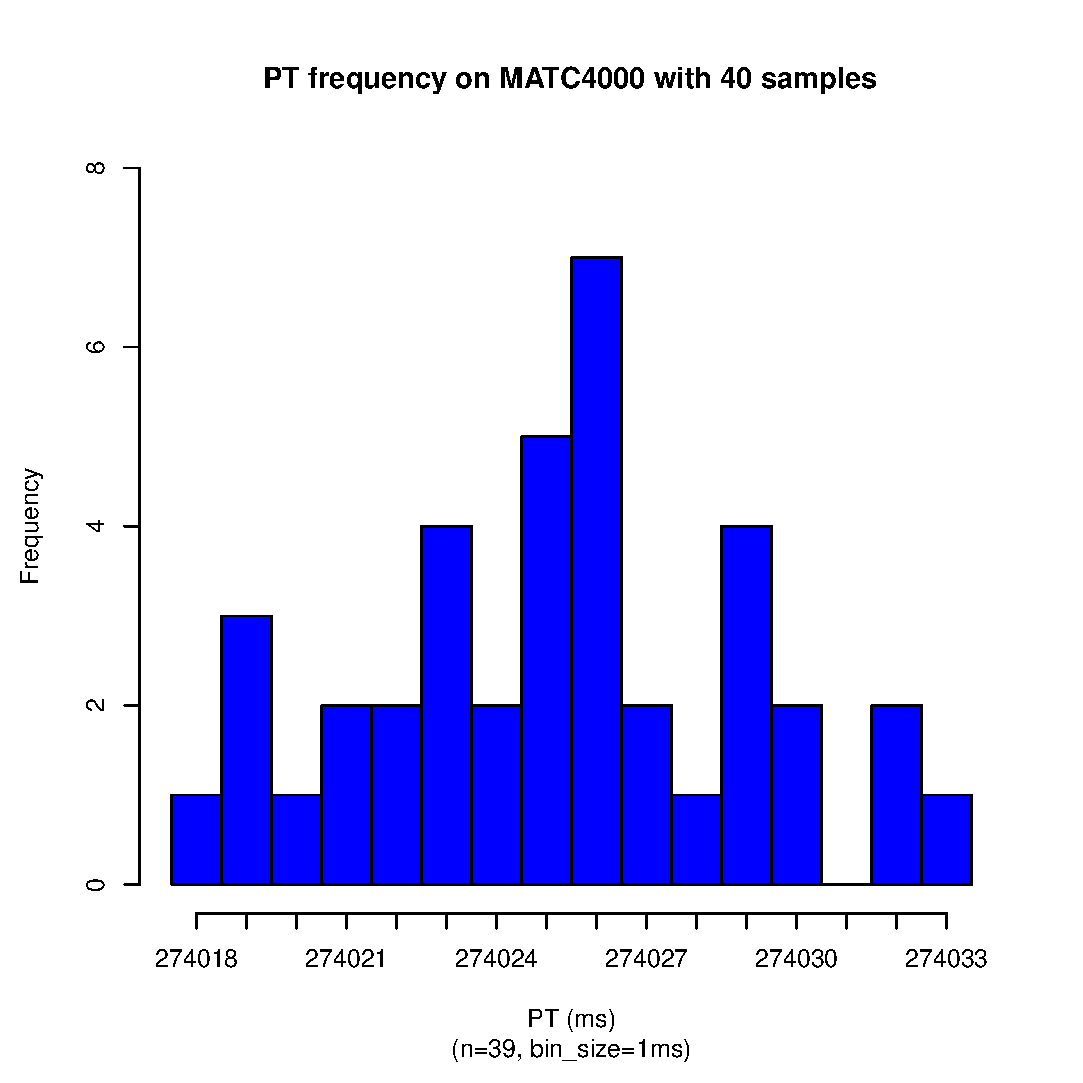
\includegraphics[scale=0.43]{matc4000_dist.eps}
		\label{fig:matc400_dist}
	}
	\subfigure[PT frequency on MATC8000]{
		\includegraphics[scale=0.43]{matc8000_dist.eps}
		\label{fig:matc800_dist}
	}
	\caption{PT Histograms of MATC1000 ... MATC8000~\label{fig:matc}}
\end{figure}

\subsubsection{Row Major}

Figure~\ref{fig:matc} shows a series of 
histograms of the execution times measured on 
the same matrix multiplication program in row major 
as the input sizes grows from 1K$\times$1K to 8K$\times$8K by the steps of 2{\small $\times$}. 

\pagebreak

\begin{figure}[h]
	\centering
	\subfigure[PT frequency on MATR1000]{
		\includegraphics[scale=0.43]{matr1000_dist.eps}
		\label{fig:matr100_dist}
	}
	\subfigure[PT frequency on MATR2000]{
		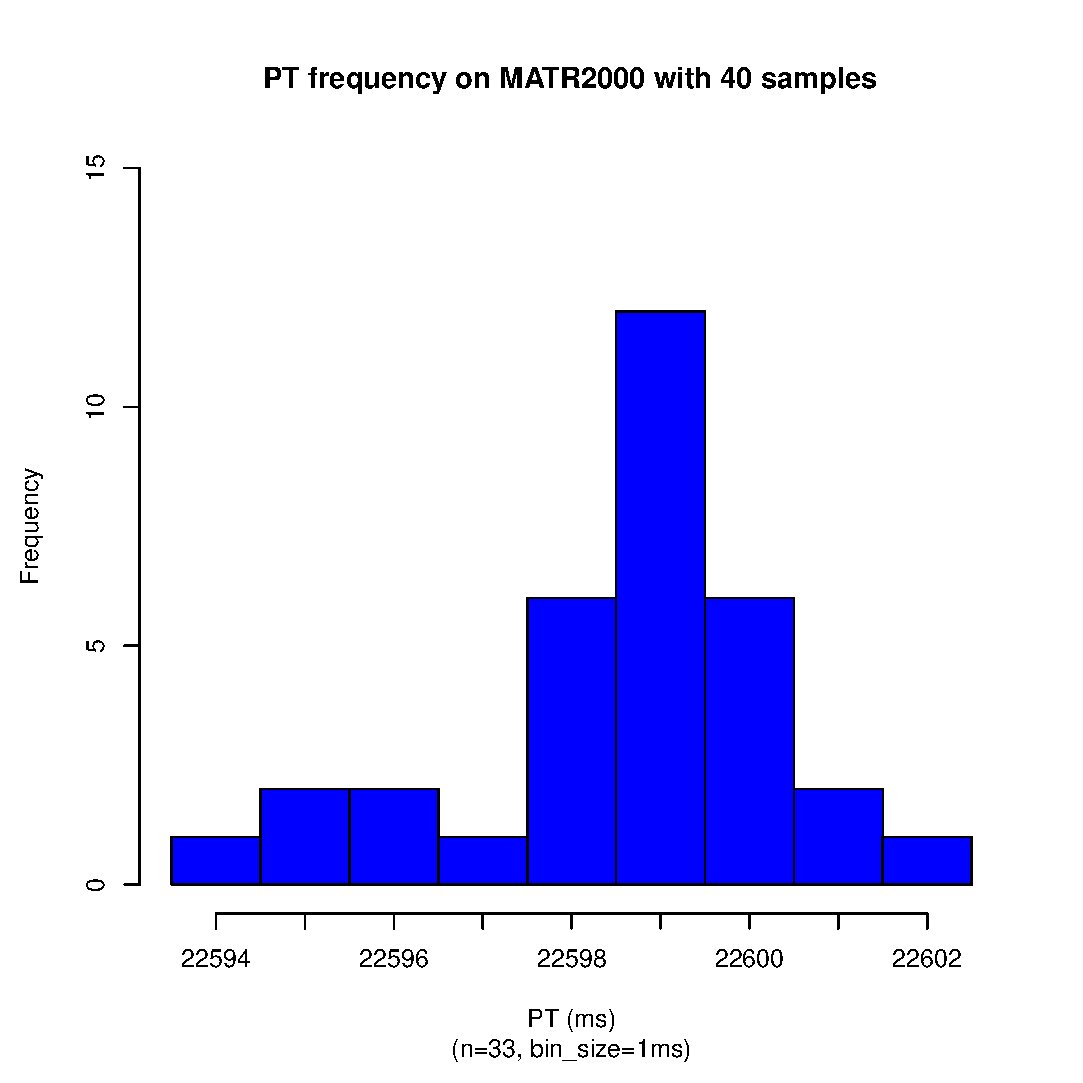
\includegraphics[scale=0.43]{matr2000_dist.eps}
		\label{fig:matr200_dist}
	}
	\subfigure[PT frequency on MATR4000]{
		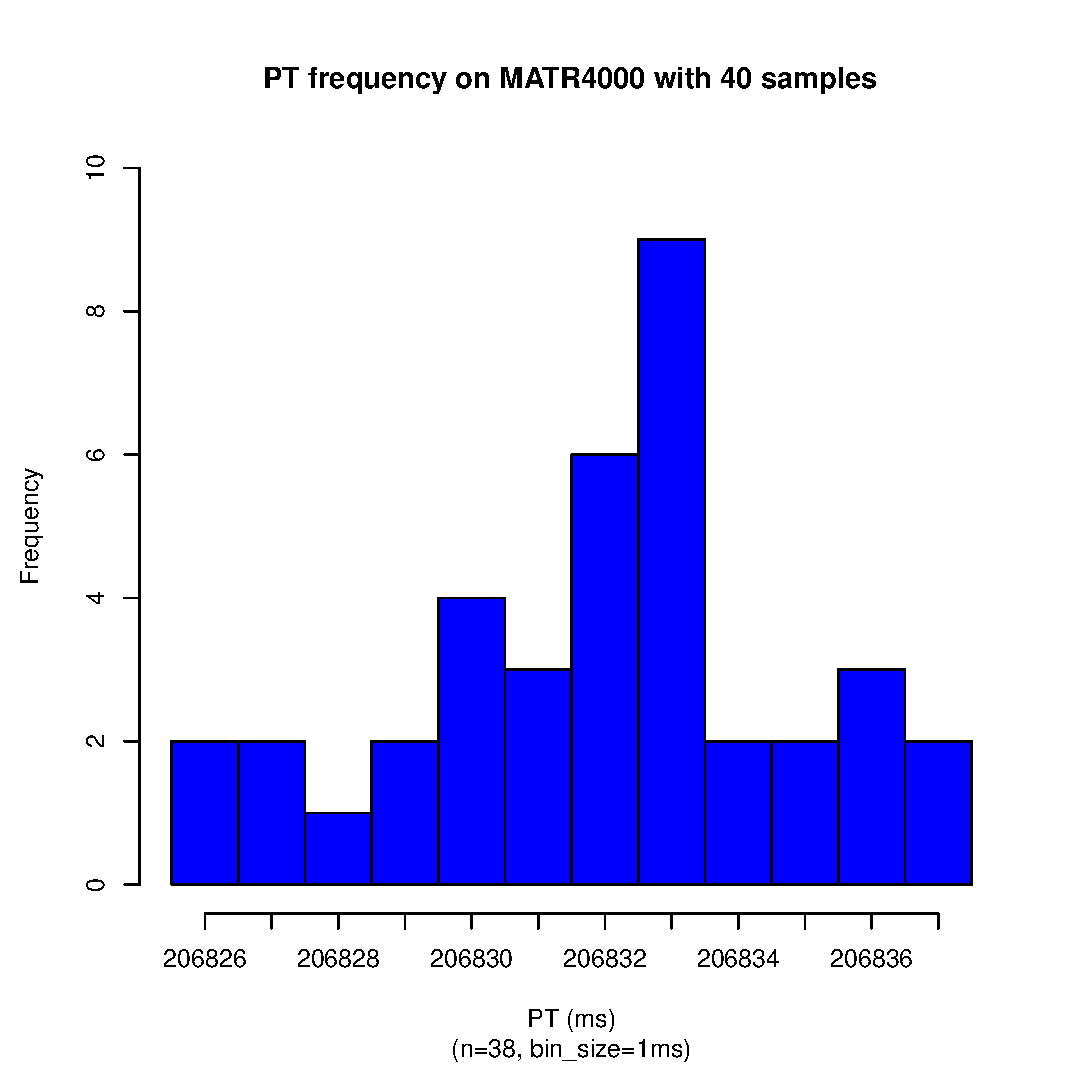
\includegraphics[scale=0.43]{matr4000_dist.eps}
		\label{fig:matr400_dist}
	}
	\subfigure[PT frequency on MATR8000]{
		\includegraphics[scale=0.43]{matr8000_dist.eps}
		\label{fig:matr800_dist}
	}
	\caption{PT Histograms of MATR1000 ... MATR8000~\label{fig:matr}}
\end{figure}

\bibliographystyle{abbrv}
\newcommand{\etalchar}[1]{$^{#1}$}
\begin{thebibliography}{99}
\vspace{0.1em}
%\bibitem
%{Avnur:2000:ECA:342009.335420}
%{Sedona}
%Young-Kyoon Suh, ``SEDONA: A Novel Protocol for Identifying Infrequent, Long-running Daemons on a Linux System'', in {\em IEICE Transactions on Information Systems}, Vol. 100D, No. 9, pp.~??--??, 2017.
%\vspace{0.1em}
\bibitem
%{Avnur:2000:ECA:342009.335420}
{EMP}
Young-Kyoon Suh, Richard T. Snodgrass, John Kececioglu, Peter J. Downey, Rob S. Maier, and Cheng Yi, ``EMP: Execution Time Measurement Protocol for Compute-Bound Programs'', in {\em Software: Practice and Experience}, 47(4):559--597, 2017.
\bibitem
%{Avnur:2000:ECA:342009.335420}
{Metrology}
Sabah Currim,Richard T. Snodgrass, Young-Kyoon Suh, and Rui Zhang, ``DBMS Metrology: Measuring Query Time'', in {\em ACM Transactions on Database Systems}, 42(1):3:1--42(+8), 2017.
\end{thebibliography}

\end{document}